\documentclass[notitlepage]{report}

\title{
	\textsc{ \small
		Physics 415
	} \\
	{\textsc{\small Lab \#3}} \\
	Quantum Eraser
}
\author{Kevin Evans \\ Partner: Sierra Ray}
\date{March 2, 2021}
\usepackage{amssymb}
\usepackage{mathtools}

\usepackage{amsthm}
\usepackage{amsmath}
\usepackage{slashed}
\usepackage{relsize}
\usepackage{threeparttable}
\usepackage{float}
\usepackage{booktabs}
\usepackage{boldline}
\usepackage{changepage}
\usepackage{physics}
\usepackage[inter-unit-product =\cdot]{siunitx}
\usepackage{setspace}
\usepackage{caption}
\usepackage{subcaption}
\usepackage[makeroom]{cancel}
%\usepackage{pgfplots}

\usepackage{enumitem}
\usepackage{times}
\usepackage{titling} % for titlingpage environment
\usepackage{calligra}
\usepackage{graphicx}
\DeclareMathAlphabet{\mathcalligra}{T1}{calligra}{m}{n}
\DeclareFontShape{T1}{calligra}{m}{n}{<->s*[2.2]callig15}{}
\newcommand{\scriptr}{\mathcalligra{r}\,}
\newcommand{\boldscriptr}{\pmb{\mathcalligra{r}}\,}
\newcommand{\emf}{\mathcal{E}}
\renewcommand{\thesection}{\arabic{section}}

\begin{document}
	\begin{titlingpage}
		\maketitle
		\begin{abstract}
			\noindent A polarization exercise was completed where Malus' law was verified using a HeNe laser and a photodetector, where a polarizer was placed in between the relative intensity was recorded as a function of the angle. 
			
			A Mach Zehnder interferometer was constructed with a HeNe laser initially polarized at \SI{45}{\deg}, with polarizers on each arm. With equal polarizations on each arm, an interference pattern was observed. Cross polarizing the arms resulted in no interference pattern. After adding an additional polarizer at \SI{45}{\deg}, the interference pattern was again observed. This additional polarizer is known as the \textit{quantum eraser}, and effectively removes the ``which path'' information encoded by the orthogonal polarizers.
		\end{abstract}
	\end{titlingpage}
	
	\section{Description of Experiment}
	This experiment was divided into two parts: first, an exercise determining the intensity of a polarizer relative to its angle, second the quantum eraser experiment was demonstrated using a Mach-Zehnder interferometer. Four polarizers were used and their polarization angles were initially recorded.
	
	\subsubsection{Polarizer exercise}
	On the optical breadboard, a ``z'' was created, creating a parallel beam from the HeNe laser. A photodiode terminated with a \SI{100}{\kohm} resistor was attached to a multimeter and placed in line with the beam. A polarizer was placed in front of the photodiode. The polarizer was rotated every \SI{20}{\deg} between $0$ and \SI{180}{\deg}, and the corresponding voltages were recorded and plotted in Origin.
	
	Next, an additional polarizer was placed between the polarizer and the laser, in a crossed polarizer configuration. The second polarizer was rotated in \SI{20}{\deg} increments on the same range, and the corresponding voltages were recorded and plotted in Origin.
	
	\subsubsection{Quantum eraser}
	A Mach-Zehnder interferometer was constructed on the optical breadboard. Shown in Figure \ref{fig:setup}, a polarizer at \SI{45}{\deg} was placed in front of the HeNe laser path. Initially, the interferometer was aligned such that an interference pattern appeared on the screen. The screen was placed roughly \SI{1}{\m} from the second beamsplitter plate, allowing an easy ``beamwalk.'' 
	
	\begin{figure}[h]
		\centering
		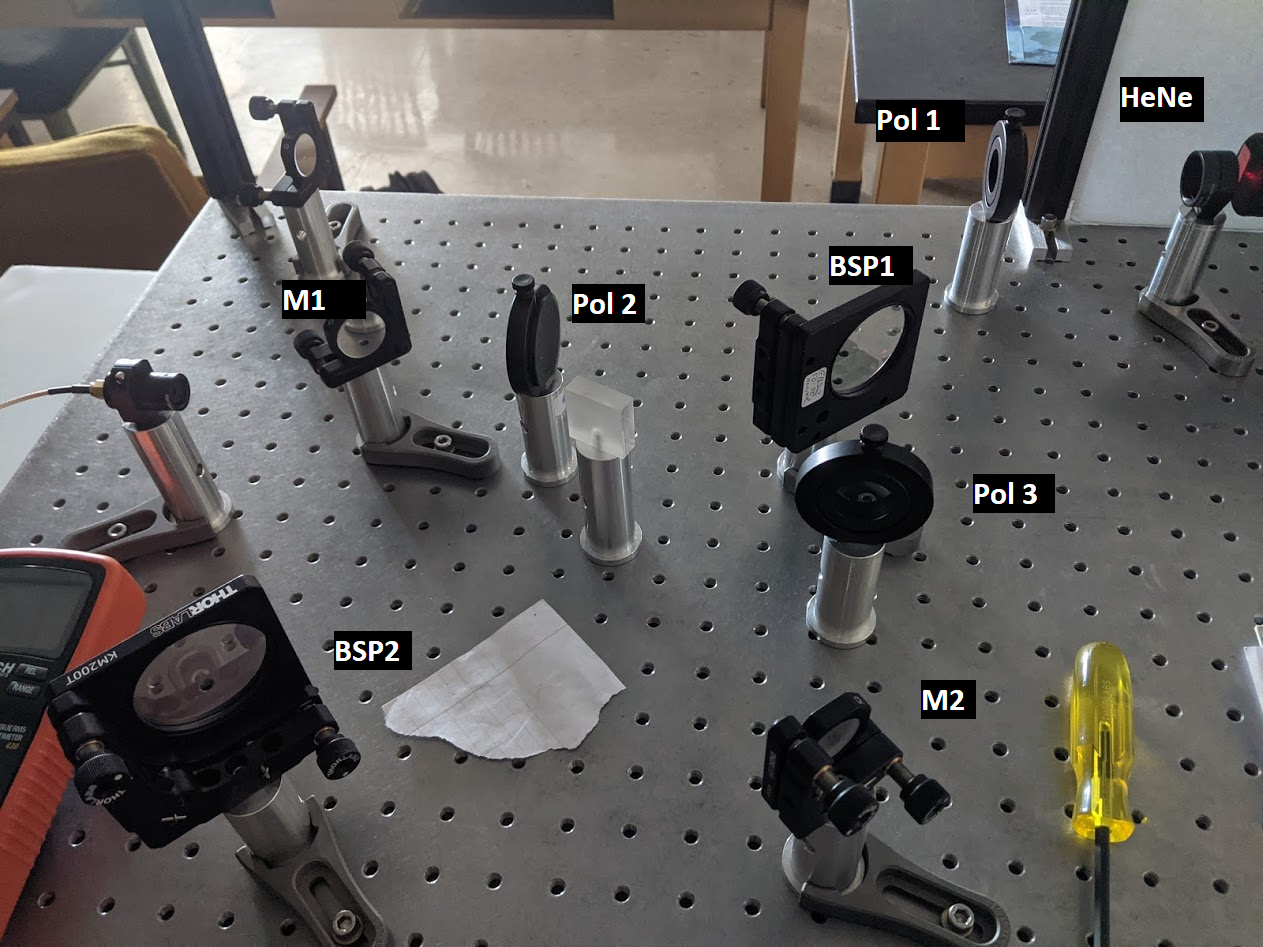
\includegraphics[width=0.7\linewidth]{setup}
		\caption{The experimental setup of the Mach-Zehnder interferometer. Pol. 4 is not shown.}
		\label{fig:setup}
	\end{figure}
	
	A vertically-oriented polarizer was placed at each arm of the interferometer and an interference pattern was observed on the screen.
	Next, one polarizer was rotated to a horizontal orientation and the screen was observed. Then without rotating the polarizers on the breadboard, an additional polarizer was placed at the output of the interferometer. Three configurations were tested: vertical, horizontal, and 45 deg. 
	

	\section{Data and Analysis}
	Initially, the orientation of the four polarizers used were recorded, shown in Table \ref{table:polarization_angles}. The angles recorded cross-polarized the incident light from the HeNe laser, which is assumed to be vertically polarized. 
	
	\begin{table}[h]
		\centering
		\caption{Cross polarization angles of the polarizers used.}
		\label{table:polarization_angles}
		\begin{tabular}{cc}
			\toprule
			Polarizer & Cross Polarization Angle [\si{\deg}] \\
			\midrule
			1 & $90.5$ \\
			2 & $90.0$ \\
			3 & $86.0$ \\
			4 & $89.0$ \\
			\bottomrule
		\end{tabular}
	\end{table}
	
	\subsubsection{Polarizer exercise}
	The polarizer was rotated every \SI{20}{\deg}. The photodiode voltages were recorded, shown in Table \ref{table:polarizerex}, then plotted in Origin, shown in Figure \ref{fig:graph1}. Applying a sine fit results in \begin{equation}
		V(\theta) = 114.4 + 114.9 \sin(\pi \frac{\theta - 134.9}{86.8}) \qquad [\si{\mV}] \label{eq:sinefit}
	\end{equation}
	
	\begin{figure}[p]
		\centering
		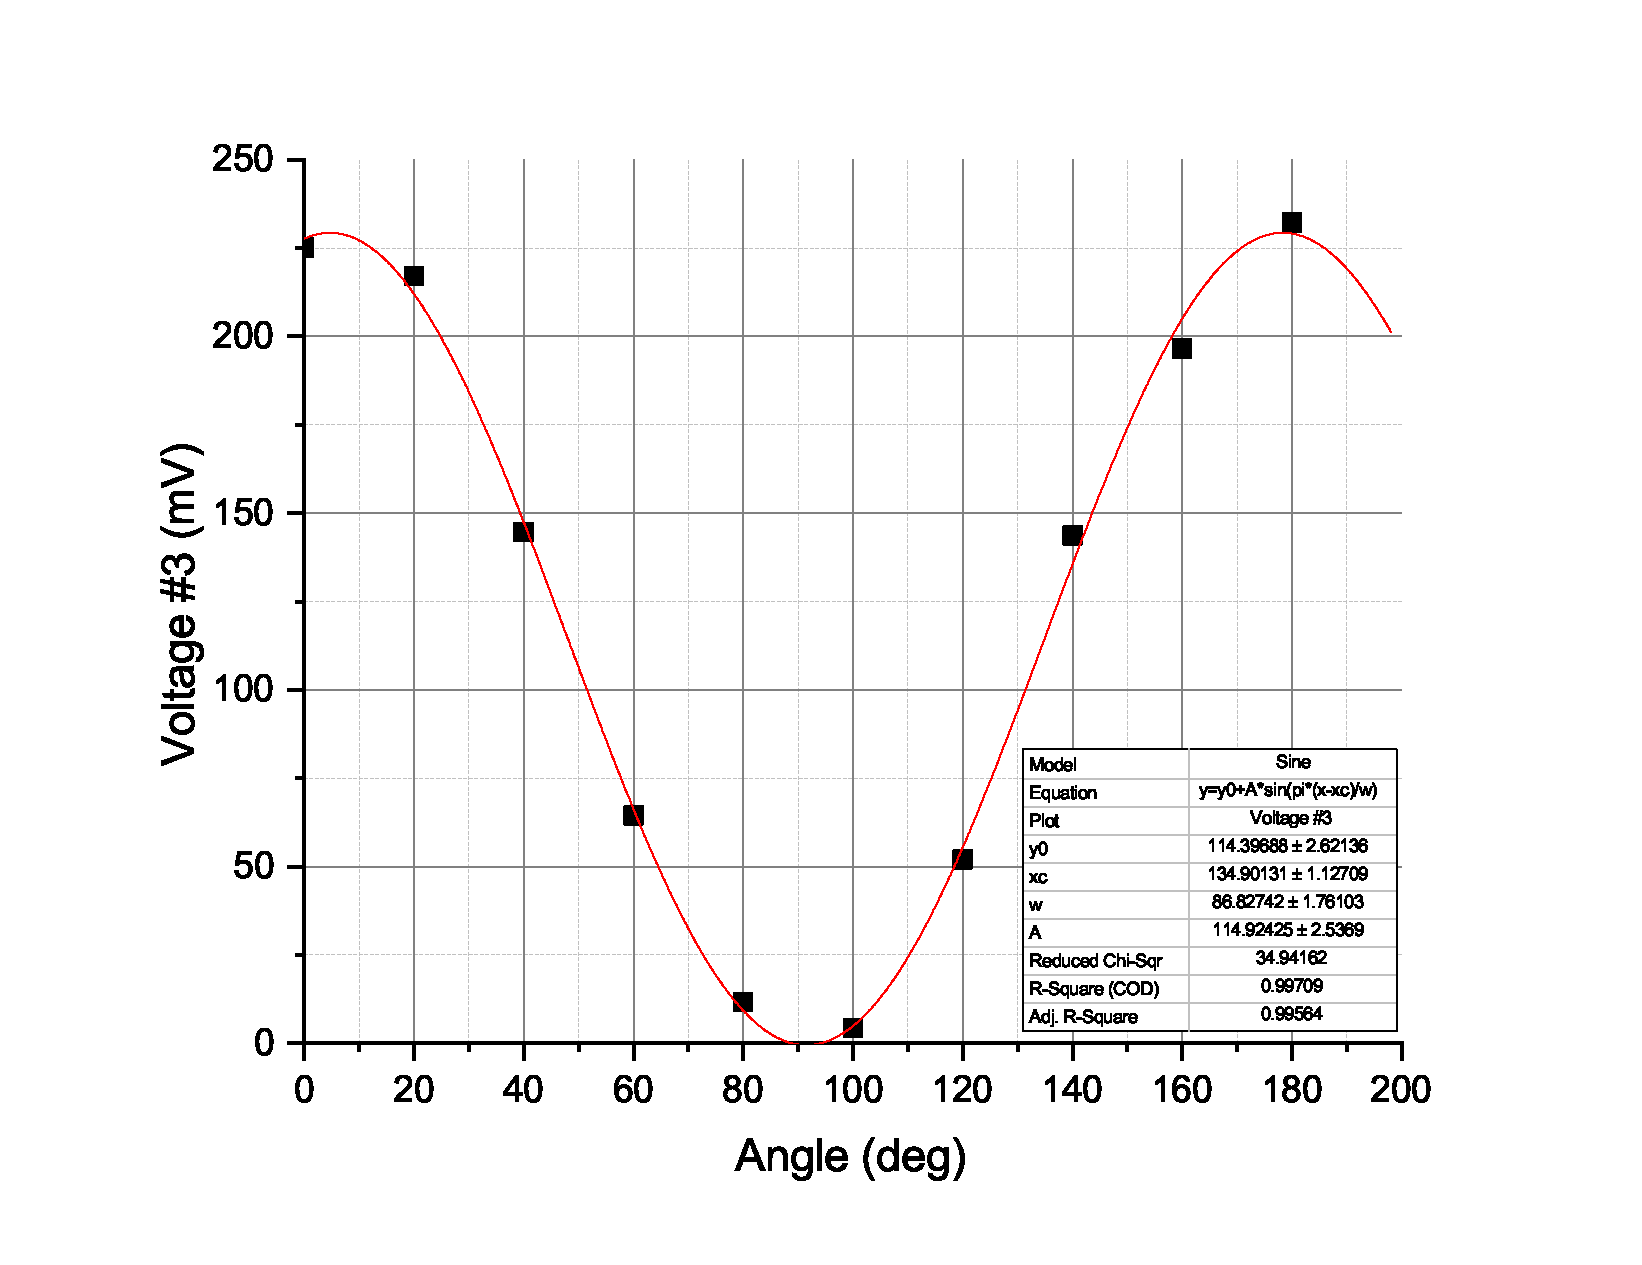
\includegraphics[width=0.9\linewidth]{Graph1}
		\caption{The intensity as a function of the polarizer rotation angle $\theta$.}
		\label{fig:graph1}
	\end{figure}
	
	\begin{figure}[p]
		\centering
		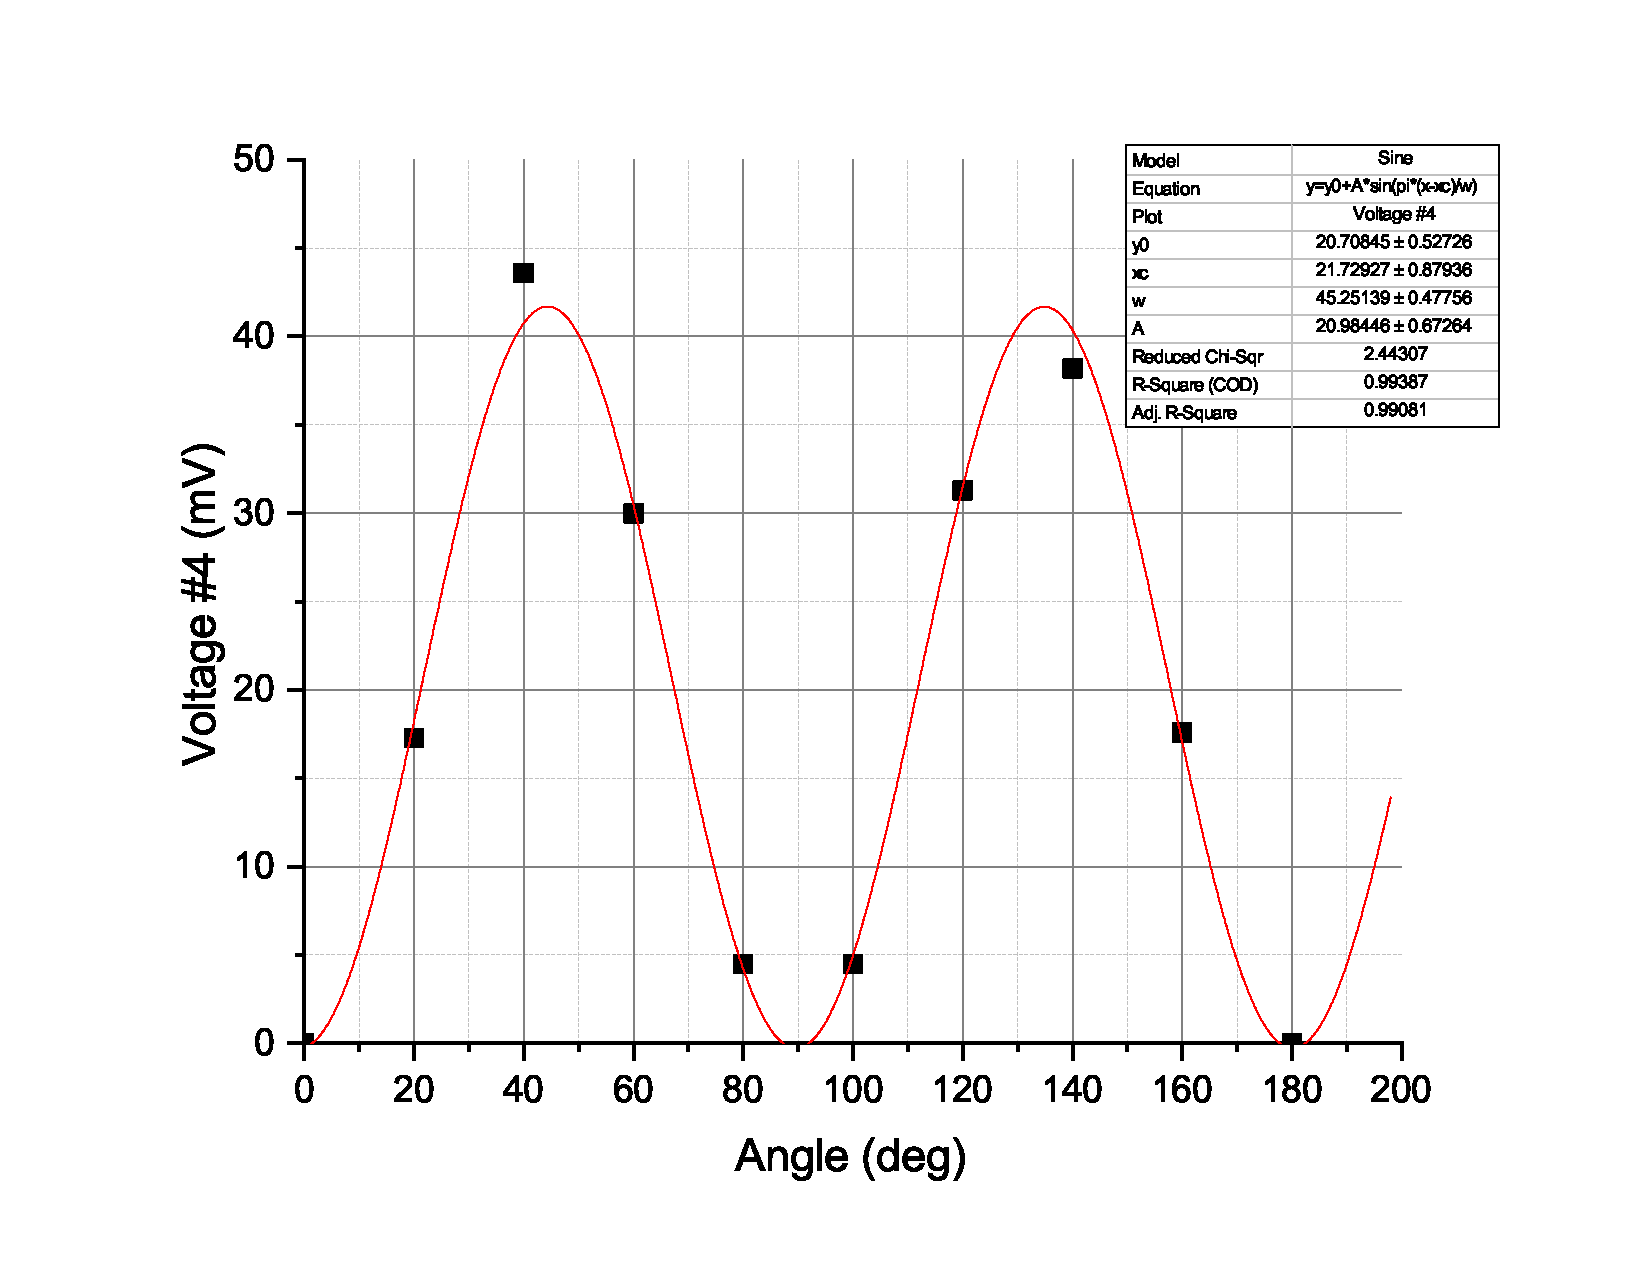
\includegraphics[width=0.9\linewidth]{Graph2}
		\caption{The intensity measured after a cross-polarized polarizer is rotated.}
		\label{fig:graph2}
	\end{figure}
	Next, after adding the additional polarizer, the data was collected, shown in Table \ref{table:polarizerex}, then plotted with a sine fit in Figure \ref{fig:graph2}.
	
	\subsubsection{Quantum eraser}
	After constructing the Mach-Zender interferometer and completing a ``beam walk'', an interference pattern was seen. Next, a vertically-aligned polarizer was placed in each arm of the interferometer, resulting in an interference pattern shown in Figure \ref{fig:interference1}. 
	
	\begin{figure}[p]
		\begin{minipage}{0.5\linewidth}
		\centering
		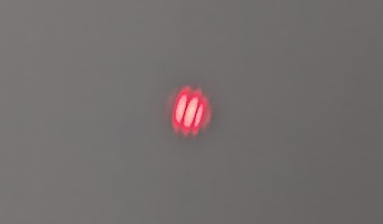
\includegraphics[width=\linewidth]{interference1}
		\caption{The initial interference pattern by the Mach-Zehnder interferometer.}
		\label{fig:interference1}
		\end{minipage}
	\hfill
	\begin{minipage}{0.48\linewidth}
	\centering
	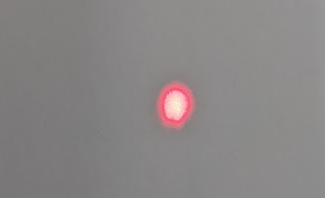
\includegraphics[width=\linewidth]{interference2}
	\caption{No interference when each arm is orthogonally polarized.}
	\label{fig:interference2}
	\end{minipage}

\vspace{2em}

\begin{minipage}{0.5\linewidth}
	\centering
	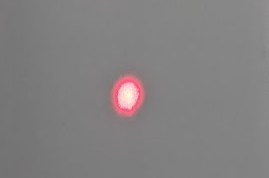
\includegraphics[width=\linewidth]{interference3}
	\caption{No interference when the quantum eraser polarizer is horizontal or vertical.}
	\label{fig:interference3}
\end{minipage}
\hfill
\begin{minipage}{0.48\linewidth}
	\centering
	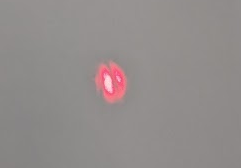
\includegraphics[width=\linewidth]{interference4}
	\caption{An interference pattern shown when the quantum eraser is at 45 deg.}
	\label{fig:interference4}
\end{minipage}
	\end{figure}

	
	After adjusting one polarizer to be horizontally oriented (and the other polarizer remaining vertical), the interference pattern disappeared and a single dot appeared on the screen, shown in Figure \ref{fig:interference2}.
	

	A polarizer was placed at the output of the interferometer and was rotated to three orientations: horizontal, vertical, and 45 deg polarizations. The horizontal and vertical polarization did not result in an interference pattern, shown by Figure \ref{fig:interference3}. However, the 45 deg polarization created an interference pattern on the screen, shown in Figure \ref{fig:interference4}.
	


	
	\section{Results and Conclusion}
	The polarizer exercise resulted in a sinusodial plot for the intensity as a function of time. The sinusoidal fit agrees with Malus' law, where the intensity $I$ is \begin{equation}
		I = I_0 \cos[2](\theta)
	\end{equation}
	In the model \eqref{eq:sinefit}, a sine function was fitted. This can be described as a squared cosine, as \[ \cos[2](\theta) = \frac{1 + \sin(\pi / 2 - 2 \theta)}{2} \]
	Applying our model to Malus' law, the maximum intensity $I_0$ is \SI{229.8}{\mV}.
	
	After adding the second polarizer, initially cross-polarized, no light was detected. As we rotated the polarizer, the light was detected again in a sinusoidal pattern. From a classical view of light, the additional polarizer only polarizes a component of the incident light, then transmits it in a new polarization. Since the polarizer is transmitting the light at a new angle, there exists a component of the light that is no longer cross-polarized.
	
	\subsubsection{Quantum eraser}
	Initially, the Mach Zehnder interferometer shows an interference pattern as both arms of the light have equal polarization and an unknown ``which path'' state until the photons hit the screen.
	
	After polarizing each arm separately, with one arm horizontally and one arm vertically polarized, the interference pattern disappears. There is no interference as each polarizer collapses the photon's unknown path, and effectively labels each state with a polarization. As the photon crosses a polarizer, the path is known and can no longer interfere with itself. From a classical view, this can be explained as two orthogonal polarizations cannot interfere.
	
	Next, a polarizer was placed at the output of the interferometer. When the polarizer is horizontally or vertically polarized, only photons from a single arm of the interferometer are transmitted. The photons from the arm which has an orthogonal polarization are blocked.
	
	However, when the polarizer is at 45 deg, both photons are able to pass through and the previous polarization state is now lost. At this point, the photons can cause interference with itself, effectively erasing the quantum information encoded by the crossed polarizers.
	
	
	\pagebreak
	\section*{Data tables}
	\begin{table}[h]
		\centering
		\caption{The relative intensities of the photodetector as a function of the polarizer angle during the polarizer exercise.}
		\label{table:polarizerex}
		\begin{tabular}{ccc}
			\toprule
			Angle [\si{\deg}] & Voltage (\#3) [\si{\mV}] & Voltage (\#4) [\si{\mV}] \\
			\midrule
			0           & 225.3         & 0             \\
			20          & 217.2         & 17.3          \\
			40          & 144.8         & 43.6          \\
			60          & 64.5          & 30            \\
			80          & 11.7          & 4.5           \\
			100         & 4.4           & 4.5           \\
			120         & 52.1          & 31.3          \\
			140         & 143.8         & 38.2          \\
			160         & 196.6         & 17.6          \\
			180         & 232.3         & 0             \\
			\bottomrule
		\end{tabular}
	\end{table}

	\begin{center}
		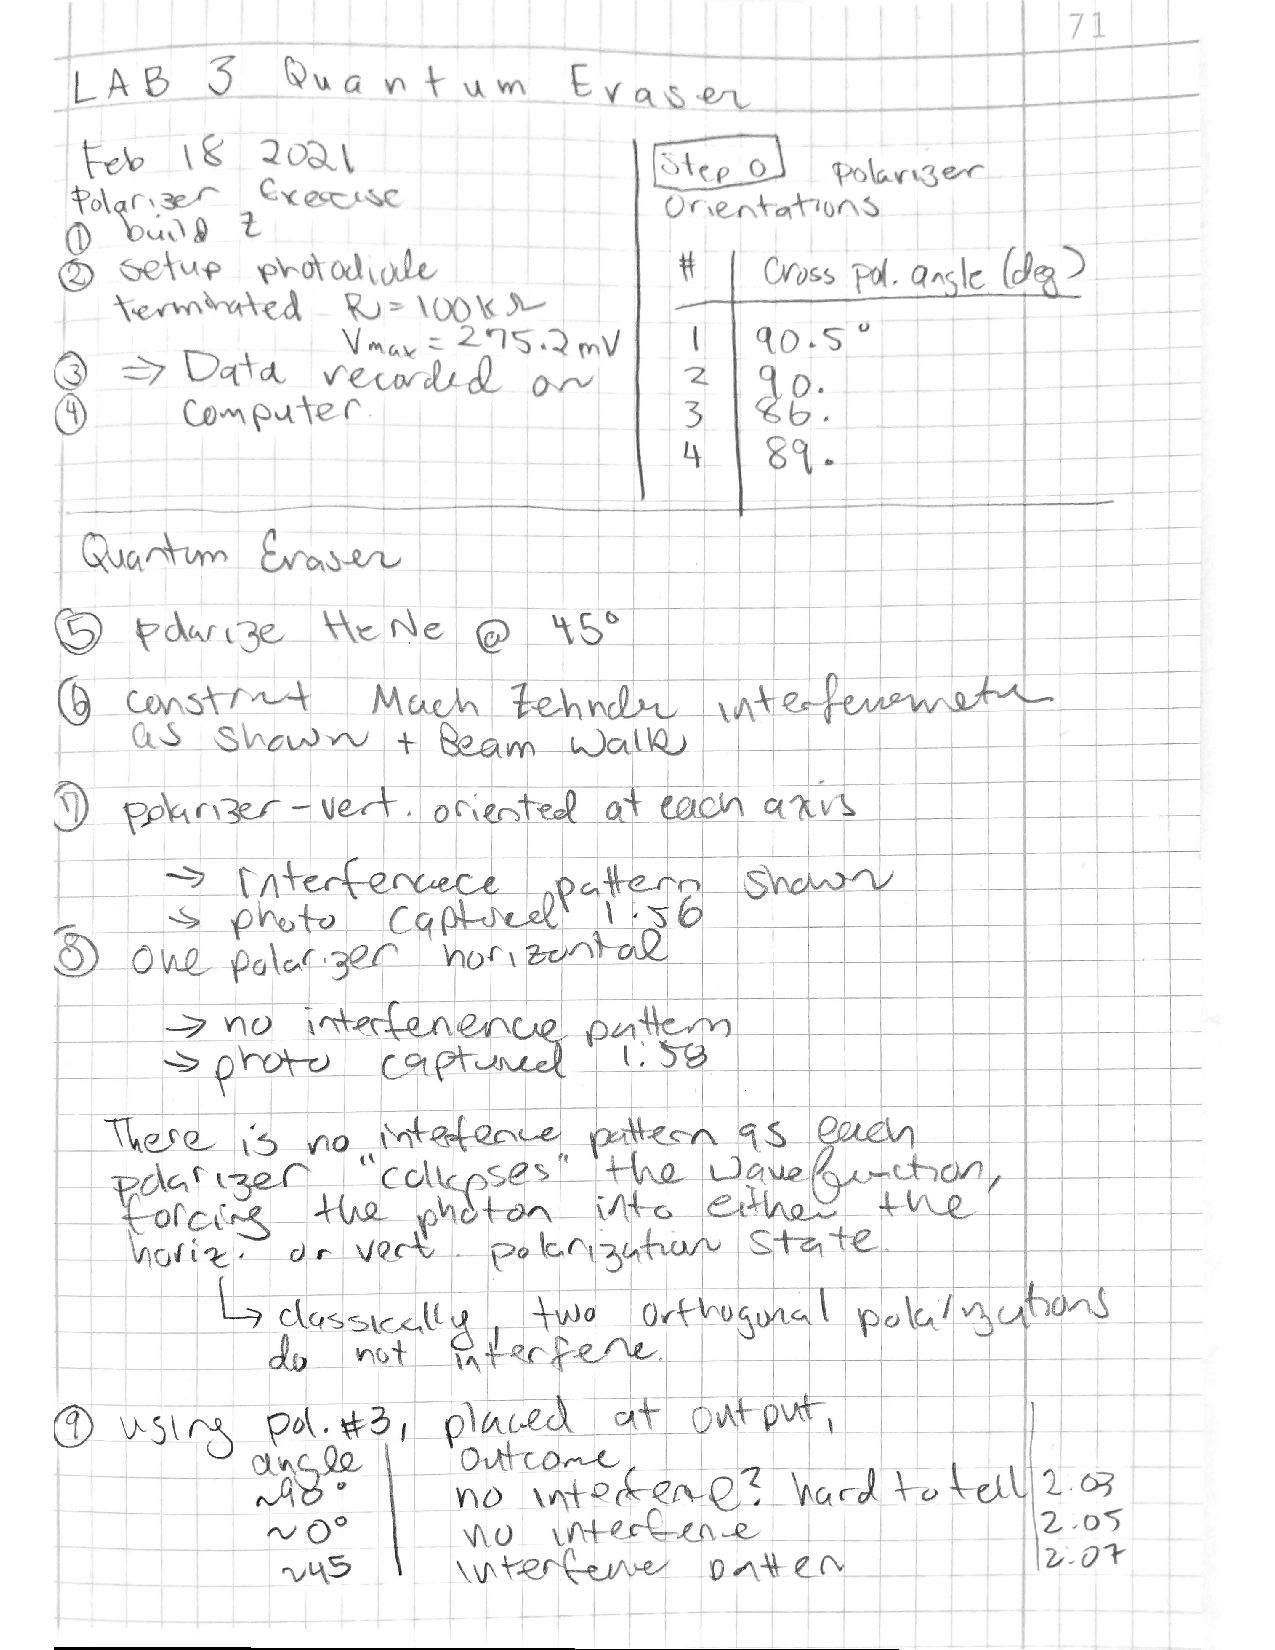
\includegraphics[width=\linewidth]{Scanned_20210302-1405}
	\end{center}
	
\end{document}